\section{Experiments}
\label{sec:experiments}

To show the efficiency of mathematical optimization with {\tt ensmallen}, we
compare its performance with several other commonly used optimization
frameworks, including some that use automatic differentiation.

\begin{figure}[t!]
\hrule
\vspace{1ex}
\begin{minted}{c++}
#include <ensmallen.hpp>

struct RosenbrockFunction
{
  template<typename MatType>
  static typename MatType::elem_type Evaluate(const MatType& x) const
  {
    return 100 * std::pow(x[1] - std::pow(x[0], 2), 2) + std::pow(1 - x[0], 2);
  }
};

int main()
{
  // We use Armadillo's timing functionality to print how long it takes to optimize.
  arma::wall_clock clock;

  RosenbrockFunction rf;
  ens::ExponentialSchedule sched;
  // A tolerance of 0.0 means the optimization will run for the maximum number of iterations.
  ens::SA<> s(sched, 100000, 10000, 1000, 100, 0.0);

  // Get the initial point of the optimization.
  arma::mat parameters = rf.GetInitialPoint();

  // Run the optimization and time it.
  clock.tic();
  s.Optimize(rf, parameters);
  const double time = clock.toc();
  std::cout << time << std::endl << "Result (optimal 1, 1): " << parameters.t();
}
\end{minted}
\hrule
\vspace*{-0.5em}
\caption{Code to use {\tt ensmallen} to optimize the Rosenbrock function using
100K iterations of simulated annealing.}
\label{fig:rosenbrock_run}
\end{figure}

\subsection{Simple optimizations and overhead}

For our first experiment, we aim to capture the overhead involved in various
optimization toolkits.  In order to do this, we consider the simple and popular
Rosenbrock function~\cite{Rosenbrock1960}:
%
\begin{equation}
f([x_1, x_2]) = 100 (x_2 - x_1^2)^2 + (1 - x_1^2).
\end{equation}

This objective function is useful for this task because the computational effort
involved in computing $f(\cdot)$ is trivial.  Therefore, if we hold the number
of iterations of each toolkit constant, then this will help us understand the
overhead costs of each toolkit.  For the optimizer, we use simulated
annealing~\cite{kirkpatrick1983optimization}, a gradient-free optimizer.
Simulated annealing will call the objective function numerous times; for each
simulation we limit the optimizer to 100K objective evaluations.

The code used to run this simulation for {\tt ensmallen} (including the
implementation of the Rosenbrock function) is given in
Figure~\ref{fig:rosenbrock_run}.  Note that the {\tt RosenbrockFunction} is
actually implemented in {\tt ensmallen}'s source code, in the directory {\tt
include/ensmallen\_bits/problems/}.

% TODO: code snippet comparison for each language?

We compare four frameworks for this task:
%
\begin{itemize}
\itemsep=-1ex
  \item[{\bf (i)}] {\tt ensmallen},
  \item[{\bf (ii)}] {\tt scipy.optimize.anneal} from SciPy 0.14.1~\cite{jones2014scipy},
  \item[{\bf (iii)}] simulated annealing implementation in {\tt Optim.jl} with Julia 1.0.1~\cite{mogensen2018optim},
  \item[{\bf (iv)}] {\tt samin} in the {\tt optim} package for Octave~\cite{octave}.
\end{itemize}

While another option here might be {\tt simulannealbnd()}
in the Global Optimization Toolkit for MATLAB,
no license was available.
We ran our code on a MacBook Pro i7 2018 with 16GB RAM running macOS 10.14 with clang 1000.10.44.2, Julia version 1.0.1, Python 2.7.15, and Octave 4.4.1.

Our initial implementation for each toolkit, corresponding to the line
``default'' in Table~\ref{tab:rosenbrock_results}, was as simple of an
implementation as possible and included no tuning.  This reflects how a typical
user might interact with a given framework.  Only Julia and {\tt ensmallen} are
compiled, and thus are able to avoid the function pointer dereference for
evaluating the Rosenbrock function and take advantage of inlining and related
optimizations.  The overhead of both {\tt scipy} and {\tt samin} are quite
large---{\tt ensmallen} is nearly three orders of magnitude faster for the same
task.

\begin{table}[t!]
\begin{center}
\begin{tabular}{lcccc}
\toprule
 & {\tt ensmallen} & {\tt scipy} & {\tt Optim.jl} & {\tt samin} \\
\midrule
default & {\bf 0.004s} & 1.069s & 0.021s & 3.173s \\
tuned & & 0.574s & & 3.122s \\
\bottomrule
\end{tabular}
\end{center}
\vspace*{-0.5em}
\caption{Runtimes for $100$K iterations of simulated annealing with various
frameworks on the simple Rosenbrock function.  Julia code runs do not count
compilation time.  The {\it tuned} row indicates that the code was manually
modified for speed.}
\label{tab:rosenbrock_results}
\end{table}

% Actually Octave's JIT is apparently some kind of prototype joke and it doesn't
% even compile anymore.  So MEX was the only way...
However, both Python and Octave have routes for acceleration,
such as Numba~\cite{lam2015numba}, MEX bindings and JIT compilation.
We hand-optimized the Rosenbrock implementation using Numba,
which required significant modification of the
underlying \texttt{anneal.anneal()} function.
These techniques did produce some speedup,
as shown in the second row of Table~\ref{tab:rosenbrock_results}.
For Octave, a MEX binding did not produce a noticeable difference.
We were unable to tune either \texttt{ensmallen} or \texttt{
Optim.jl} to get any speedup, suggesting that novice users will easily be able
to write efficient code in these cases.

\subsection{Large-scale linear regression problems}

\begin{table}[t!]
\centering
%\begin{adjustbox}{scale={0.90}{0.90}}
\begin{tabular}{lccccc}
\toprule
{\em algorithm} & $d$: 100, $n$: 1k & $d$: 100, $n$: 10k & $d$: 100, $n$:
100k & $d$: 1k, $n$: 100k \\
\midrule
\texttt{ensmallen}-1 & {\bf 0.001s} & {\bf 0.009s} & {\bf 0.154s} & {\bf 2.215s} \\
\texttt{ensmallen}-2 & 0.002s & 0.016s & 0.182s & 2.522s \\
% Dropped for space and awful performance
%\texttt{Calculus.jl} & 0.172s & 0.960s & 27.428s & 2535.507s \\
\texttt{Optim.jl} & 0.006s & 0.030s & 0.337s & 4.271s \\
\texttt{scipy} & 0.003s & 0.017s & 0.202s & 2.729s \\
\texttt{bfgsmin} & 0.071s & 0.859s & 23.220s & 2859.81s\\
% It's possible to tune ForwardDiff.jl a bit, but it doesn't give significant
% speedups to make it competitive and it really makes the code ugly.
\texttt{ForwardDiff.jl} & 0.497s & 1.159s & 4.996s & 603.106s \\
\texttt{autograd} & 0.007s & 0.026s & 0.210s & 2.673s \\
\bottomrule
\end{tabular}
%\end{adjustbox}
\vspace*{0.25ex}
\caption{
Runtimes for the linear regression function on various dataset sizes,
with $n$ indicating the number of samples,
and $d$ indicating the dimensionality of each sample.
All Julia runs do not count compilation time.}
\label{tab:lbfgs}
\end{table}

Next, we consider the linear regression example described in
Sec.~\ref{sec:linreg_example}.  For this task we use the first-order L-BFGS
optimizer~\cite{liu1989limited}, implemented in {\tt ensmallen} as the {\tt
L\_BFGS} class.  Using the same four packages, we implement
the linear regression objective and gradient.  Remembering that {\tt ensmallen}
allows us to share work across the objective function and gradient
implementations (Section~\ref{sec:automatic}), for {\tt ensmallen} we implement
a version with only {\tt EvaluateWithGradient()}, denoted as {\tt ensmallen-1}.
We also implement a version with both \texttt{Evaluate()} and
\texttt{Gradient()}: \texttt{ensmallen-2}.  We also use automatic
differentiation for Julia via the \texttt{
ForwardDiff.jl}~\cite{RevelsLubinPapamarkou2016} package and for Python via the
\texttt{Autograd}~\cite{maclaurin2015autograd} package.  For GNU Octave
we use the \texttt{bfgsmin()} function.

Results for various data sizes are shown in Table~\ref{tab:lbfgs}.  For each
implementation, L-BFGS was allowed to run for only $10$ iterations and never
converged in fewer iterations.  The datasets used for training are highly noisy random
data with a slight linear pattern. Note that the exact data is not relevant
for the experiments here, only its size.  Runtimes are reported as the
average across 10 runs.

The results indicate that \texttt{ensmallen} with
\texttt{EvaluateWithGradient()} is the fastest approach.
Furthermore, the use of \texttt{EvaluateWithGradient()} yields
non-negligible speedup over the \texttt{ensmallen-2} implementation with
both the objective and gradient implemented separately.  In addition, although
the automatic differentiation support makes it easier for users to write their
code (since they do not have to write an implementation of the gradient), we
observe that the output of automatic differentiators is not as efficient,
especially with \texttt{ForwardDiff.jl}.  We expect this effect to be
more pronounced with increasingly complex objective functions.

\subsection{Easy pluggability of various optimizers}

Lastly, we demonstrate the easy pluggability in \texttt{ensmallen}
for using various optimizers on the same task.
Using a version of {\tt LinearRegressionFunction} from
Section~\ref{sec:linreg_example} adapted for separable differentiable
optimizers, we run six optimizers with default parameters in just 8 lines of
code, as shown in Fig.~\ref{fig:learning_curve_code}.
Applying these optimizers to the \texttt{YearPredictionMSD}
dataset from the UCI repository~\cite{ucimlrepository}
yields the learning curves shown in Fig.~\ref{fig:learning_curve}(b).

\begin{figure}[t!]
\hrule
\vspace{1ex}
\begin{minted}{c++}
// X and y are data.
LinearRegressionFunction lrf(X, y);

using namespace ens;
StandardSGD<>().Optimize(lrf, sgdModel);
Adam().Optimize(lrf, adamModel);
AdaGrad().Optimize(lrf, adagradModel);
SMORMS3().Optimize(lrf, smorms3Model);
SPALeRASGD().Optimize(lrf, spaleraModel);
RMSProp().Optimize(lrf, rmspropModel);
\end{minted}
\hrule
\vspace*{-0.5em}
\caption{{\tt ensmallen} makes it easy to switch out optimizer types: 8
lines of code run 6 different optimizers on one problem.}
\label{fig:learning_curve_code}
\end{figure}

Any other optimizer for separable differentiable objective
functions can be dropped into place in the same manner; given {\tt ensmallen}'s
large number of available optimizers, this support could be used to easily
compare optimizers.  In fact, this is exactly done with the interactive
optimizer visualization tool found at \url{https://vis.ensmallen.org}.
Figure~\ref{fig:visualization} shows an example visualization from that page.

\begin{figure}[t!]
  \vspace*{-1em}
  \centering
  % 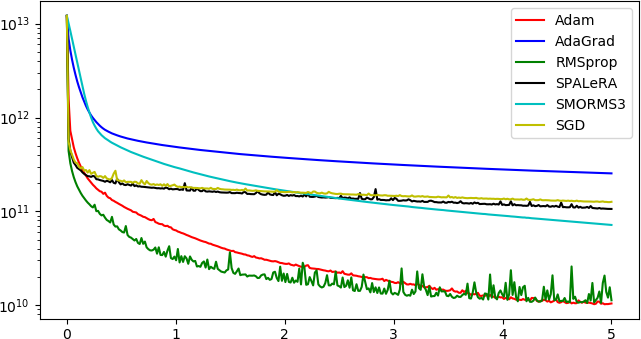
\includegraphics[width=\textwidth,height=0.45\textwidth]{experiments/learning_curves_crop.png}
  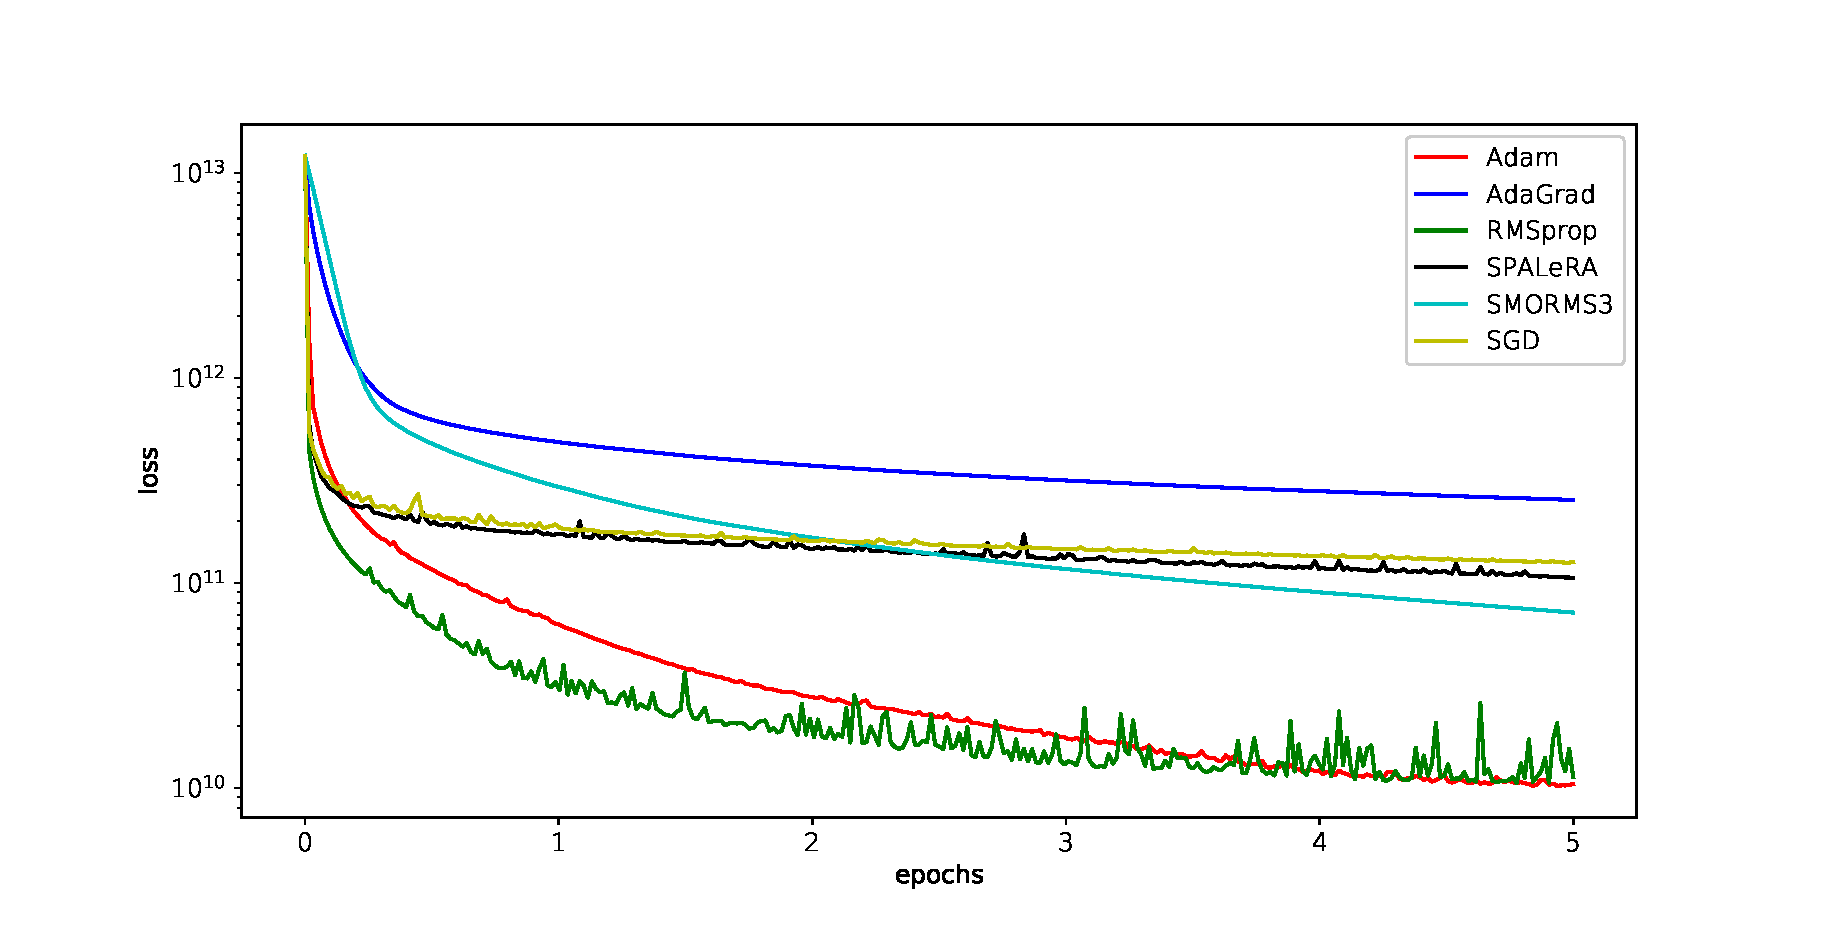
\includegraphics[width=\textwidth,height=0.5\textwidth]{experiments/learning_curves_crop.eps}
  %% CS: to remove the blank space around the plot:
  %% CS: epstool --copy --bbox input.eps output.eps
  \vspace*{-2.5em}
\caption{
Example usage of six {\tt ensmallen} optimizers to optimize a linear regression
function on the {\tt YearPredictionMSD} dataset~\cite{ucimlrepository} for 5
epochs of training.  The optimizers can be tuned for better performance.}
\label{fig:learning_curve}
\end{figure}

\begin{figure}[t!]
  \centering
  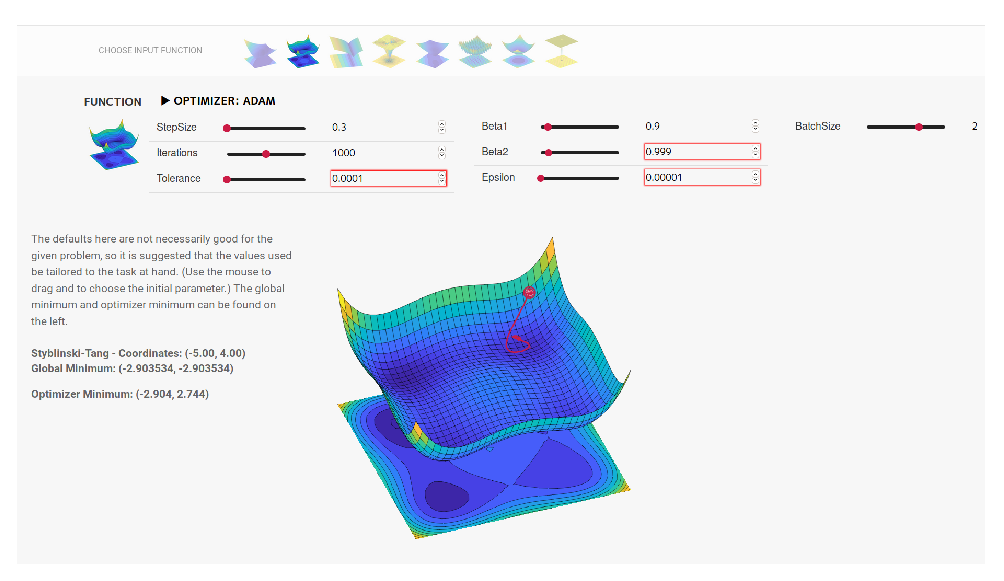
\includegraphics[width=\textwidth]{experiments/visualization.eps}
  \vspace*{-2em}
  \caption{Visualization of the Adam optimizer on the Styblinski-Tang objective
function; this is a screen capture from \url{https://vis.ensmallen.org}.}
  \label{fig:visualization}
\end{figure}

